\documentclass[a4paper]{article}
\usepackage{hyperref}
\usepackage{graphicx}
\usepackage[dvipsnames]{xcolor}
\usepackage{listings}

\lstset{
  frame=single,
  rulecolor=\color{black},
  breaklines=true,
  breakatwhitespace=false,
  postbreak=\mbox{\textcolor{gray}{$\hookrightarrow$}\space},
  basicstyle=\ttfamily\small,
  columns=fullflexible,
  keywordstyle=\color{Blue}\bfseries,
  stringstyle=\color{ForestGreen},
  commentstyle=\color{Gray}\itshape
}

\makeatletter
\newcommand{\pydifempty}[1]{%
\if\relax\detokenize\expandafter{#1}\relax
\expandafter\@firstoftwo
\else
\expandafter\@secondoftwo
\fi
}
\makeatother

% pydocmaker:parameters:begin
% NOTE: parameter names use a leading "p" (pTitle, pAuthor, ...) so the derived
% LaTeX macros (\pTitle, ...) never collide with LaTeX kernel macros.
% pydocmaker:param:pTitle
\providecommand{\pTitle}{Pydocmaker Documentation}
% pydocmaker:param:pAuthor
\providecommand{\pAuthor}{Tobias Glaubach}
% pydocmaker:param:pDate
\providecommand{\pDate}{}
% pydocmaker:param:pAcronyms
\providecommand{\pAcronyms}{}
% pydocmaker:param:pApplicables
\providecommand{\pApplicables}{}
% pydocmaker:param:pReferences
\providecommand{\pReferences}{}
% pydocmaker:param:pSubtitle
\providecommand{\pSubtitle}{Automatically created via pydocmaker from README.md}
% pydocmaker:param:pHideToc
\providecommand{\pHideToc}{false}
% pydocmaker:param:pDocCategory
\providecommand{\pDocCategory}{Report}
% pydocmaker:param:pHideDate
\providecommand{\pHideDate}{false}
% pydocmaker:param:pTitlepageInfoDict
\newcommand{\pTitlepageInfoDict}{%
\begin{description}
\item{Version}{v2.8.0}
\item{Repository}{https://github.com/TobiasGlaubach/pydocmaker}
\item{Documentation}{https://pydocmaker.readthedocs.io}
\end{description}
}
% pydocmaker:param:pHidePydocmaker
\providecommand{\pHidePydocmaker}{false}
% pydocmaker:param:pAbstract
\providecommand{\pAbstract}{A minimal python document maker to create and show reports (including figures and tables) from within python and export them to markdown, pdf, html, and word.}
% pydocmaker:param:pHeaderStrLeft
\providecommand{\pHeaderStrLeft}{https://pypi.org/project/pydocmaker/ v2.8.0 documentation}
% pydocmaker:param:pHeaderStrRight
\providecommand{\pHeaderStrRight}{2026-11-23}
% pydocmaker:param:pVersion
\providecommand{\pVersion}{v2.8.0}
% pydocmaker:parameters:end

\begin{document}

\pydifempty\pTitle{}{\begin{center}{\LARGE \textbf{\pTitle}}\end{center}}

\pydifempty\pAuthor{}{\begin{center}{\large \pAuthor}\end{center}}

\pydifempty\pDate{}{\begin{center}{\pDate}\end{center}}

\pydifempty\pAcronyms{}{\section*{List of Acronyms}\pAcronyms}

\pydifempty\pApplicables{}{\section*{Applicable Documents}\pApplicables}

\pydifempty\pReferences{}{\section*{Reference Documents}\pReferences}

% pydocmaker:body:begin
\section{pydocmaker}\label{pydocmaker}

\begin{figure}
\centering
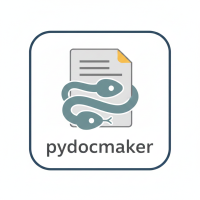
\includegraphics{icon.png}
\caption{Icon}
\end{figure}

A minimal easy to use python document maker to create reports in \passthrough{\lstinline!pdf!}, \passthrough{\lstinline!md!}, \passthrough{\lstinline!typst!}, \passthrough{\lstinline!html!}, \passthrough{\lstinline!docx!}, \passthrough{\lstinline!tex!} and more formats. Written purely in python, but optional features use external non python libraries such as \passthrough{\lstinline!typst!} or pandoc (if installed). Nearly no code written by AI (some test cases, and some documentation was written by AI tools)

\begin{itemize}
\tightlist
\item
  \textbf{NOTE:} some functions will try to call pandoc and fall back if not found.
\item
  \textbf{NOTE:} exporting PDFs by default works using \passthrough{\lstinline!typst!}. All other engines need optional dependencies, such as either a latex compiler or Microsoft Word, or Libreoffice.
\end{itemize}

Full documentation at https://pydocmaker.readthedocs.io/en/latest/

For an \textbf{example of a created PDF document} please see \passthrough{\lstinline!README.pdf!} (located within the root folder of this repository) which is this \passthrough{\lstinline!README.md!} file converted to pdf via \passthrough{\lstinline!pydocmaker!} and \passthrough{\lstinline!typst!} with the \passthrough{\lstinline!report!} template.

\subsection{Installation}\label{installation}

Install via:

\begin{lstlisting}[language=bash]
pip install pydocmaker
\end{lstlisting}

\subsection{TL;DR; Code examples}\label{tldr-code-examples}

\subsubsection{Snippet:}\label{snippet}

\begin{lstlisting}[language=Python]

import pydocmaker as pyd

doc = pyd.Doc.get_example()
doc.show()
\end{lstlisting}

\subsubsection{Minimal Usage Example:}\label{minimal-usage-example}

\begin{lstlisting}[language=Python]

import pydocmaker as pyd

doc = pyd.Doc() # basic doc. Workd like a list, We always append new content to the end
doc.add('dummy text') # adds raw text

# this is how to add parts to the document
doc.add_pre('this will be shown as preformatted') # preformatted
doc.add_md('This is some *fancy* `markdown` **text**') # markdown
doc.add_tex(r'\textbf{Hello, LaTeX!}') # latex
doc.add_table([['John Doe', "30"]], header=['Name', 'Age'], caption='example table') # table

# this is how to add an image from link
doc.add_image("https://github.githubassets.com/assets/GitHub-Mark-ea2971cee799.png", caption='Github Logo')

# this is how to add matplotlib figures to your report
import matplotlib.pyplot as plt
fig = plt.figure()
plt.plot([1,2,3], [6,5,7])
doc.add_image(fig, caption='Example figure', width=0.7)

# show will render and show a doc when in an iPython
# environment such as jupyter or colab, on the terminal 
# it will fall back to use rich console instead
doc.show()
\end{lstlisting}

\subsubsection{``Showing'' Documents in iPython/Terminal}\label{showing-documents-in-ipythonterminal}

the \passthrough{\lstinline!Doc!} class has a method called \passthrough{\lstinline!show!} which will detect if its running in \passthrough{\lstinline!Ipython!}. If it does it will render the document and show it. If not it will fallback to a rich consiole and do its best to show the content on the terminal (on a terminal image support is very limited). The desired rendering format can be set with the \passthrough{\lstinline!engine!} argument. \passthrough{\lstinline!rich!}, \passthrough{\lstinline!markdown!}, \passthrough{\lstinline!HTML!}, or \passthrough{\lstinline!PDF!} is possible.

Any environment: \textbf{NOTE}: when rendering with ``rich'' console image support is very limited, since images will be printed on the console as pixels (with the size being scaled down to the console width)

\begin{lstlisting}[language=Python]
doc.show()
doc.show('rich')
doc.show('rich', embed_images=False)
\end{lstlisting}

In \passthrough{\lstinline!Ipython!} (such as Jupyter or Colab) any of the following:

\begin{lstlisting}[language=Python]
doc.show('md')
\end{lstlisting}

Or:

\begin{lstlisting}[language=Python]
doc.show('html')
\end{lstlisting}

Or:

\begin{lstlisting}[language=Python]
doc.show('pdf')
\end{lstlisting}

\textbf{NOTE}: some IDEs do not support the PDF option and instead open a ``save'' dialog, but in a browser with jupyter this works

\subsubsection{Exporting:}\label{exporting}

export via:

\begin{lstlisting}[language=Python]
# returns string
text_html = doc.export('html')
# or write a file
doc.export('path/to/my_file.html')
\end{lstlisting}

Or alternatively:

\begin{lstlisting}[language=Python]
doc.to_html('path/to/my_file.html') # will write a HTML file
doc.to_pdf('path/to/my_file.pdf') # will write a PDF file via typst
doc.to_pdf('path/to/my_file.zip') # will write the whole latex project dir as a pdf file
doc.to_markdown('path/to/my_file.md') # will write a Markdown file
doc.to_docx('path/to/my_file.docx') # will write a docx file
doc.to_textile('path/to/my_file.textile.zip') # will pack all textile files and write them to a zip archive
doc.to_tex('path/to/my_file.tex.zip') # will pack all tex files and write them to a zip archive
doc.to_ipynb('path/to/my_file.ipynb') # will write a ipynb file

doc.to_json('path/to/doc.json') # saves the document
\end{lstlisting}

\subsubsection{Saving and Loading (Minimal)}\label{saving-and-loading-minimal}

A minimal example showing how to save and load \passthrough{\lstinline!Doc!} objects. \passthrough{\lstinline!Doc.save!} accepts a file path (string or \passthrough{\lstinline!pathlib.Path!}) or a file-like object. When no path is provided it returns the rendered content (HTML by default). \passthrough{\lstinline!Doc.load!} accepts a JSON string/bytes, a path, or a stream.

\begin{lstlisting}[language=Python]
import pydocmaker as pyd

doc = pyd.get_example()

# save to common formats (case-insensitive suffixes are supported)
doc.save('report.html')      # writes HTML
doc.save('report.json')      # writes JSON
doc.save('report.ipynb')     # writes an ipynb (may depend on environment)

doc2 = pyd.load('report.json') # load back in (should now be same as doc)

json_str = doc.save(format='json') # save as in-memory string in given format
loaded = pyd.load(json_str) # and load back

\end{lstlisting}

Supported save/load formats for \passthrough{\lstinline!Doc.save!}/\passthrough{\lstinline!Doc.load!}:

\begin{itemize}
\tightlist
\item
  \passthrough{\lstinline!.html!}, \passthrough{\lstinline!.pyd!}, \passthrough{\lstinline!.pydoc!} --- HTML serialization/serialization used by pydocmaker
\item
  \passthrough{\lstinline!.ipynb!} --- Jupyter notebook (may require additional environment support)
\item
  \passthrough{\lstinline!.json!} --- Raw document JSON (recommended for round-trip fidelity)
\end{itemize}

\textbf{Note}: Saving and Loading is fundamentally different from exporting a report (e.G. to\_html), since save/load allows round trip loading and saving, while exporting makes nice documents to view in other other software and not load again.

\subsubsection{Configuring Options:}\label{configuring-options}

All configurable options for this package are in \passthrough{\lstinline!pydocmaker.options!}. They are always callable functions with ``*\_get'', ``*\_set'', ``*\_scan'' etc.

\begin{lstlisting}[language=Python]

import pydocmaker as pyd

pyd.options.pandoc_allowed_set(False)
print(pyd.options.pandoc_allowed_get())

pyd.options.pdf_engine_set('typst') # default
print(pyd.options.pdf_engine_get())
\end{lstlisting}

\subsubsection{Block Templates (comment-delimited, standalone-compilable)}\label{block-templates-comment-delimited-standalone-compilable}

Besides the classic Jinja2 templates (\passthrough{\lstinline!.j2!} files), pydocmaker supports \textbf{block templates}: plain \passthrough{\lstinline!.html!}, \passthrough{\lstinline!.tex!} and \passthrough{\lstinline!.typ!} files that carry \passthrough{\lstinline!pydocmaker:!} markers inside comments. These files stay valid and compilable standalone (the native compilers ignore the parameter constructs and show the body placeholder) while pydocmaker can render, scaffold and update them without ever modifying the file on disk during render.

\begin{lstlisting}[language=TeX]
% pydocmaker:parameters:begin
% pydocmaker:param:title
\providecommand{\title}{My Report}
% pydocmaker:param:acronyms
\newcommand{\acronyms}{%
\begin{description}
\item{SNR}{Signal-to-Noise Ratio}
\end{description}
}
% pydocmaker:parameters:end

\begin{document}
% pydocmaker:body:begin
placeholder text
% pydocmaker:body:end
\end{document}
\end{lstlisting}

\begin{lstlisting}
// pydocmaker:parameters:begin
// pydocmaker:param:title
#let title = "My Report"
// pydocmaker:param:acronyms
#let acronyms = (SNR: "Signal-to-Noise Ratio")
// pydocmaker:parameters:end

// pydocmaker:body:begin
placeholder text
// pydocmaker:body:end
\end{lstlisting}

\begin{lstlisting}[language=HTML]
<!-- pydocmaker:parameters:begin -->
<!-- pydocmaker:param:title -->
<meta name="pydocmaker:param:title" content="My Report">
<!-- pydocmaker:parameters:end -->
<body>
<!-- pydocmaker:body:begin -->
placeholder text
<!-- pydocmaker:body:end -->
</body>
\end{lstlisting}

Engine selection is automatic (markers in the template source select the block engine) and can be forced with the \passthrough{\lstinline!template\_engine!} argument (\passthrough{\lstinline!'auto'!} (default), \passthrough{\lstinline!'jinja2'!} or \passthrough{\lstinline!'blocks'!}) on \passthrough{\lstinline!Doc.to\_html!}, \passthrough{\lstinline!Doc.to\_typst!} and \passthrough{\lstinline!Doc.to\_pdf!}:

\begin{lstlisting}[language=Python]
import pydocmaker as pyd

doc = pyd.Doc().add_text('Hello Block Templates')

# auto-detection: marked sources render through the block engine
out = doc.to_typst(template='my_template.typ', template_params={'title': 'Rendered'})

# explicit override
out = doc.to_typst(template='my_template.typ', template_engine='blocks')
out = doc.to_typst(template='my_template.typ', template_engine='jinja2')
\end{lstlisting}

The \passthrough{\lstinline!pydocmaker.blocktmpl!} subpackage exposes the engine directly:

\begin{lstlisting}[language=Python]
from pydocmaker import blocktmpl

blocktmpl.detect(source)                    # True if block markers are present
blocktmpl.parse(source, tformat='typ')      # parse into a BlockDocument
blocktmpl.scaffold(source, tformat='typ', params={'title': 'V1'})   # insert missing blocks
blocktmpl.update_params(source, {'title': 'V2'})                    # write values back (idempotent)
blocktmpl.render(source, body='...', params={'title': 'V2'})        # replace body + apply params
\end{lstlisting}

When resolved from a template directory, an \textbf{exact file name} (\passthrough{\lstinline!'base.tex'!}) resolves to the block file even when a \passthrough{\lstinline!base.tex.j2!} twin exists; \textbf{short IDs} (\passthrough{\lstinline!'base'!}) keep preferring the \passthrough{\lstinline!.j2!} file for backward compatibility. Shipped examples: \passthrough{\lstinline!base.tex!}, \passthrough{\lstinline!base.html!}, \passthrough{\lstinline!base.typ!} in \passthrough{\lstinline!src/pydocmaker/templates/!}.

NOTE for LaTeX templates: parameter names that collide with LaTeX kernel macros (\passthrough{\lstinline!title!}, \passthrough{\lstinline!author!}, \passthrough{\lstinline!date!}) produce inert \passthrough{\lstinline!\\providecommand!} definitions; use names such as \passthrough{\lstinline!reporttitle!} when the value shall be displayed in the document body.

\subsubsection{Install Optional Requirements}\label{install-optional-requirements}

\paragraph{\texorpdfstring{Optional Requirement \texttt{pandoc}}{Optional Requirement pandoc}}\label{optional-requirement-pandoc}

In order to get all functionality \passthrough{\lstinline!pandoc!} needs to be available. Please follow the recommended installation steps on the software projects webpage. For convenience the minimal installation is listed here:

On Linux (Debian/Ubuntu) install via:

\begin{lstlisting}[language=bash]
sudo apt update
sudo apt install pandoc
\end{lstlisting}

On MacOS:

\begin{lstlisting}[language=bash]
brew install pandoc
\end{lstlisting}

On Windows:

\begin{lstlisting}[language=bash]
winget install JohnMacFarlane.Pandoc
\end{lstlisting}

\subsubsection{\texorpdfstring{Optional Requirement \texttt{Latex}}{Optional Requirement Latex}}\label{optional-requirement-latex}

In order to get all functionality a latex compiler needs to be available. Please follow the recommended installation steps on the webpage. For convenience the minimal installation is listed here:

On Linux (Debian/Ubuntu) install via:

\begin{lstlisting}[language=bash]
sudo apt update
sudo apt install texlive-full
\end{lstlisting}

On MacOS:

\begin{lstlisting}[language=bash]
brew install --cask mactex
\end{lstlisting}

On Windows:

\begin{lstlisting}[language=bash]
winget install MiKTeX.MiKTeX
\end{lstlisting}

\subsubsection{\texorpdfstring{Optional Requirement for DOCX either \texttt{libreoffice} or \texttt{win32com}}{Optional Requirement for DOCX either libreoffice or win32com}}\label{optional-requirement-for-docx-either-libreoffice-or-win32com}

Some DOCX functionality need either Microsoft Windows and Microsoft Word and the \passthrough{\lstinline!win32com!} library or \passthrough{\lstinline!libreoffice!} available.

\paragraph{\texorpdfstring{Installing \texttt{pywin32} (Windows only)}{Installing pywin32 (Windows only)}}\label{installing-pywin32-windows-only}

Install via:

\begin{lstlisting}[language=bash]
pip install pywin32
\end{lstlisting}

\paragraph{\texorpdfstring{Installing \texttt{libreoffice}}{Installing libreoffice}}\label{installing-libreoffice}

On a Linux (Debian/Ubuntu) system insall via:

\begin{lstlisting}[language=bash]
sudo apt update
sudo apt-get install libreoffice
\end{lstlisting}

On MacOS:

\begin{lstlisting}[language=bash]
brew install --cask libreoffice
\end{lstlisting}

On Windows:

\begin{lstlisting}[language=bash]
winget install TheDocumentFoundation.LibreOffice
\end{lstlisting}

\textbf{NOTE}: You need to add the folder with the libreoffice executeables to PATH in windows.

\subsubsection{Writing Word docx Documents with templates and fields}\label{writing-word-docx-documents-with-templates-and-fields}

Below is an example on how to use pydocmaker to write word docx documents from format templates and also automatically ``replace'' fields (MergeFields in Word or plain text) to be filled out in the docx document with text from python.

(\textbf{NOTE}: some of the code below utilized the \passthrough{\lstinline!win32com!} api and only works on windows)

prepare a report, a template and some fields in the template:

\begin{lstlisting}[language=Python]

import pydocmaker as pyd

metadata = {
    'repno': "1234",
    "summary": "This is a nice workflow for automatically creating docx documents",
    "date": "2025-12-13",
    "comment": f"this works!",
    "author": "Me"
}

# HOWTO: 
#  Adding MergeFields In Word to replace them later: 
#    Go to Insert → Quick Parts → Field → MergeField.
templatepath = 'my/path/template.docx'
outpath = 'my/path/outfile.docx'

# get a pyd example document to show the concept
doc = pyd.get_example()
\end{lstlisting}

this is the quick and easy way using the common pydocmaker api:

\begin{lstlisting}[language=Python]
# three different examples below
docx_bts = doc.to_docx("my/path/outfile.docx", template=templatepath, template_params=metadata, use_w32=False)
docx_bts = doc.to_docx("my/path/outfile_w32.docx", template=templatepath, template_params=metadata, use_w32=True)
docx_bts = doc.to_docx("my/path/outfile_w32_comp.pdf", template=templatepath, template_params=metadata, use_w32=True, as_pdf=True, compress_images=True)
\end{lstlisting}




% pydocmaker:body:end

\end{document}
